\documentclass[specialist,
               substylefile = spbu_report.rtx,
               subf,href,colorlinks=true, 12pt]{disser}
               
\usepackage[a4paper,
            mag=1000, includefoot,
            left=3cm, right=1.5cm, top=2cm, bottom=2cm, headsep=1cm, footskip=1cm]{geometry}
\usepackage[T2A]{fontenc}
\usepackage[utf8x]{inputenc}
\usepackage[english, main=russian]{babel}
\ifpdf\usepackage{epstopdf}\fi

\usepackage{amsmath,amssymb,amsthm,amscd,amsfonts}
\usepackage{mathdots}
\usepackage{graphicx}

\newcommand\norm[1]{\left\|#1\right\|}
\DeclareMathOperator\R{\mathbb{R}}
\DeclareMathOperator\rank{\textrm{rank}\,}

\newtheorem{corollary}{Следствие}
\newtheorem{theorem}{Теорема}
\newtheorem{remark}{Замечание}
\newtheorem{lemma}{Лемма}
\newtheorem{sentence}{Предложение}
\newtheorem{definition}{Определение}
\newenvironment{formulation}{\paragraph{Формулировка.}}{\hfill}
\newenvironment{statement}{\paragraph{Постановка.}}{\hfill}

% Точка с запятой в качестве разделителя между номерами цитирований
%\setcitestyle{semicolon}

% Использовать полужирное начертание для векторов
\let\vec=\mathbf

% Нумерация подсекций в оглавлении
\setcounter{secnumdepth}{3}

% Включать подсекции в оглавление
\setcounter{tocdepth}{3}

\graphicspath{{fig/}}

%----------------------------------------------------------------
\begin{document}
	
% Название организации
\institution{%
    Санкт-Петербургский государственный университет \\
    Прикладная математика и информатика \\
    Вычислительная стохастика и статистические модели
}

%\title{Отчёт по курсовой работе}
\title{3 курс (бак.) <<Учебная практика 3 (научно-исследовательская работа)>>}

% Тема
\topic{\normalfont\scshape%
    Задачи анализа временных рядов, теория метода \\«Анализ Сингулярного Спектра» SSA\\ (Семестр 6)}

% Автор
\author{Яковлев Денис Михайлович}

% Научный руководитель
\sa       {В.\,В.~Некруткин}
\sastatus {к.\,ф.-м.\,н., доцент}

% Город и год
\city{Санкт-Петербург}
\date{\number\year}

\maketitle
\maketitle
\tableofcontents
\section{Введение}
Целью этой работы является решение теоретических и прикладных задач анализа временных рядов с применением знаний о методе SSA (Singular Spectrum Analysis), или ``Анализ Сингулярного Спектра'' (сокращенно, АСС). В ходе учебной практики будут изучены и продемонстрированы теоретическая часть метода АСС и её применение. Ознакомиться с методом АСС можно в \cite{GNZh01}, а в  \cite{Nekrutkin10} описывается теоретическая часть метода АСС.

\section{Постановка задачи}

\subsection{Метод АСС}
\label{ssect:SSA}
Остановимся сначала на том варианте метода АСС, который обсуждается в настоящей работе,  подробное
описание этого  метода
можно найти в \cite{GNZh01}.

Рассматривается вещественный \emph{сигнал} $\mathrm{H}=(h_0,\ldots, h_n,\ldots)$, причем предполагается, что ряд $\mathrm{H}$ управляется линейной
рекуррентной формулой  (ЛРФ) порядка~$d$
\begin{gather}
	\label{eq:rec_d}
	h_n = \sum\limits_{k=1}^d a_kh_{n-k}, \ \ n \geqslant d
\end{gather}
с $a_d>0$, которая является минимальной в том смысле, что  не существует ЛРФ меньшего порядка, управляющей рядом $\mathrm{H}$.
Кроме того, вводится \emph{помеха} $\mathrm{E}=(e_0,\ldots, e_n,\ldots)$ и предполагается, что наблюдается ряд $\widetilde{\mathrm{H}}_N=\mathrm{H}_N+\delta
\mathrm{E}_N$, где  $\mathrm{H}_N$ и $\mathrm{E}_N$ --- согласованные отрезки длины $N$ сигнала и помехи, а
$\delta$ является формальным параметром возмущения. Иначе говоря,
\begin{gather*}
	\mathrm{H}_N=(h_0, \ldots, h_{N-1}), \ \ \mathrm{E}_N=(e_0, \ldots, e_{N-1}) \ \ \text{и}\ \
	\widetilde{\mathrm{H}}_N=(h_0+\delta e_0, \ldots, h_{N-1}+\delta e_{N-1}).
\end{gather*}
Общая задача состоит в (приближенном) выделении сигнала $\mathrm{H}_N$ из суммы $\widetilde{\mathrm{H}}_N$, причем предполагается, что известно только
значение порядка $d$ ЛРФ \eqref{eq:rec_d}.
В первую очередь нас будет интересовать оценка ряда $\mathrm{H}_N$.
\paragraph{Краткое описание метода.}
Метод АСС в этом случае выглядит следующим образом.
\begin{enumerate}
	\item
	Выбирается {\it длина окна} $L<N$ и из ряда $\widetilde{\mathrm{H}}_N$ строится ганкелева {\it траекторная} матрица $\mathbf{H}(\delta)$ размерности
	$L\times K$, $K=N-L+1$, с элементами $\mathbf{H}(\delta)=(\widetilde{h}_{i+j-2})$, $0\leqslant i<L$, $0\leqslant j<K$. При этом предполагается, что $\min(L,K)\geqslant
	d$, исходя из того, что ряд $H$ управляется ЛРФ порядка $d$
	В \cite{GNZh01} эта операция называется {\it вложением}.
	
	Если обозначить $\mathbf{H}$ и $\mathbf{E}$ ганкелевы матрицы, полученные из  рядов $\mathrm{H}_N$ и $\mathrm{E}_N$ операцией вложения $\mathcal{T}_{L, N} = \mathcal{T}$ с той же
	длиной окна $L$, то, конечно,
	${\mathbf{H}}(\delta)=\mathcal{T}(\mathrm{H}_N + \delta\mathrm{E}_N)$.
	\item
	Для матрицы $\mathbf{H}(\delta)$ вычисляется сингулярное разложение и суммируются $d$ главных (то есть соответствующих наибольшим сингулярным
	числам) элементарных матриц этого разложения. А именно, выбирается ортонормированная система собственных \emph{(левых сингулярных)} векторов $\mathbf{H}(\delta)\mathbf{H}(\delta)^\mathrm{T}$ --- $\{U_i\}_{i=1}^L$ и собственных \emph{(правых сингулярных)} векторов $\mathbf{H}(\delta)^\mathrm{T}\mathbf{H}(\delta)$ --- $\{V_i\}_{i=1}^K$, вычисляются собственные числа $\mathbf{H}(\delta)\mathbf{H}(\delta)^\mathrm{T}$ --- $\{\lambda_i\}_{i=1}^L$. Если расположить все собственные числа в \emph{неубывающем порядке} и обозначить $m$ --- число ненулевых собственных чисел, то
	\begin{gather*}
		\mathbf{H}(\delta) = \sum^m_{i=1}\sqrt{\lambda_i}U_iV_i^\mathrm{T},
	\end{gather*}
где $U_i,\,V_i$ соответствуют $\lambda_i$. Результат
 \begin{gather*}
 	\widetilde{\mathbf{H}}(\delta) = \sum^d_{i=1}\sqrt{\lambda_i}U_iV_i^\mathrm{T}.
 \end{gather*} этой операции, где $m = d$, так как образованная от ряда $H$ матрица $\mathbf{H}(\delta)$ управляется ЛРФ порядка $d$, является наилучшим приближением
	матрицы $\mathbf{H}(\delta)$ с помощью матриц ранга $d$ в норме Фробениуса, то есть
	\begin{gather*}
		\arg\min_{\mathbf{A}\in\R^{L\times K},\,\rank \mathbf{A} \leqslant d}\norm{\mathbf{H}(\delta) - \mathbf{A}}=\widetilde{ \mathbf{H}}(\delta).
	\end{gather*}
	\item
	Ищется ганкелева матрица  $\widehat{ \mathbf{H}}(\delta)$, которая является ближайшей к  $\widetilde{ \mathbf{H}}(\delta)$ в той же норме
	Фробениуса.
	В явном виде это означает, что на каждой побочной диагонали $i+j=const$ все элементы матрицы $\widetilde{ \mathbf{H}}(\delta)$ заменяются их
	средним значением. Поэтому
	в \cite{GNZh01} эта операция названа {\it диагональным усреднением}. Обозначая её $\mathcal{S}$ получим, что   $\widehat{\mathbf{H}}(\delta)=\mathcal{S} \widetilde{ \mathbf{H}}(\delta)$.
	\item
	Наконец, применяя к $\widehat{ \mathbf{H}}(\delta)$ операцию, обратную к операции вложения, приходим к {\it восстановленному} ряду $\widetilde{\mathrm{H}}_{N}(\delta)=\mathcal{T}^{-1}(\widehat{\mathbf{H}}(\delta)),$
	который объявляется приближением к сигналу $\mathrm{H}_N$.
\end{enumerate}
\section{Теоретические задачи}
\begin{statement}
Введём несколько объектов:
\begin{itemize}
	\item $\mathbf{H}$, $\mathbf{E}$ --- вещественнозначные ненулевые матрицы $\R^K \rightarrow \R^L$. Матрицу $\mathbf{H}$ будем называть \emph{траекторной матрицей сигнала} $\mathrm{H}$ , а $\mathbf{E}$ --- \emph{траекторной матрицей помехи} $\mathrm{H}$. В условиях поставленной задачи рассматривается возмущённая матрица $\mathbf{H}(\delta)$ и \emph{сигнальное подпространство}, образованное столбцами матрицы $\mathbf{H}$;
	\item  $\mathbf{A} = \mathbf{HH}^\mathrm{T}$ --- самосопряжённый неотрицательно определённый оператор $\mathbf{A}$: $\R^L \rightarrow \R^L$;
	\item $d = \rank\mathbf{H} < \min(L, K)$ - ранг матрицы $\mathbf{H}$, образованной от ряда $\mathrm{H}$, управляемого ЛРФ порядка $d$;
	\item $\Sigma$ --- набор собственных числа $\{\mu_n\}_{n=1}^L$ оператора $\mathbf{A}$. Из свойств оператора $\mathbf{A}$, $\Sigma \subset [0, +\infty)$;
	\item $\mu_{min} = \min\{\mu\in\Sigma\, |\, \mu > 0\}$;
	\item $\mathbf{I}$ --- тождественный оператор $\R^L \rightarrow \R^L$;
	\item $\mathbf{P}_0$ --- ортогональный проектор на собственное подпространство $\mathbb{U}_0$, соответствующее нулевым собственным числам $\mathbf{A}$;
	\item $\mathbf{P}^\bot_0 = \mathbf{I} - \mathbf{P}_0$ --- ортогональный проектор на $\mathbb{U}_0^\bot$, соответствующее ненулевым собственным числам;
	\item $\norm{\,\cdot\,}_{\mathrm{spec}}=\norm{\,\cdot\,}$ --- спектральная норма.
\end{itemize}
Теперь введём матрицу с возмущением $\mathbf{H}(\delta) = \mathbf{H} + \delta\mathbf{E}$. Тогда возмущение оператора $\mathbf{A}$:
\begin{equation*}
	\mathbf{A}(\delta) = \mathbf{H}(\delta)\mathbf{H}(\delta)^\mathrm{T} = \mathbf{H}\mathbf{H}^\mathrm{T} + \delta(\mathbf{H}\mathbf{E}^\mathrm{T} + \mathbf{E}\mathbf{H}^\mathrm{T}) + \delta^2\mathbf{E}\mathbf{E}^\mathrm{T}.
\end{equation*}
Положим $\mathbf{A}^{(1)} = \mathbf{H}\mathbf{E}^\mathrm{T} + \mathbf{E}\mathbf{H}^\mathrm{T}$, $\mathbf{A}^{(2)} = \mathbf{E}\mathbf{E}^\mathrm{T}$, $\mathbf{B}(\delta) = \delta\mathbf{A}^{(1)} + \delta^2\mathbf{A}^{(2)}$. Заметим, что $\mathbf{A}^{(1)}$ и $\mathbf{A}^{(2)}$ --- самосопряжённые операторы, а $\mathbf{A}(\delta)$ --- самосопряжённый неотрицательный оператор для любых $\delta\in\R$. Положим $\mathbf{B}(\delta)=\delta\mathbf{A}^{(1)} + \delta^2\mathbf{A}^{(2)}$.\\
Определим $\mathbf{S}_0$ --- матрица, псевдообратная к $\mathbf{HH}^\mathrm{T}$. Положим $\mathbf{S}_0^{(0)} = -\mathbf{P}_0$ и $\mathbf{S}_0^{(k)}=\mathbf{S}_0^k$ для $k\geqslant1$, $\norm{\mathbf{S}_0^{(k)}}=1/\mu_{min}^k$.

Далее --- рассуждения из \cite[раздел 5.3]{Nekrutkin10}.

А именно, если обозначить $r_i(N)=\widetilde{h}_i(\delta)-h_i$ --- остаток от разности между $i$-ми элементами рядов $\widetilde{\mathrm{H}}_N(\delta)\text{ и }\mathrm{H}_N$, а $\mathbf{N}(\delta) = \mathbf{N}_N(\delta)$ --- оператор с возмущением, то из того, что  $\norm{\mathbf{C}}_{\max}\leqslant \norm{\mathbf{C}}$, получаем
\begin{align*}
	&\norm{\widetilde{\mathrm{H}}_{N}(\delta) - \mathrm{H}_N}_{\max} = \max_{0\leqslant n<N}|\widetilde{h}_n(\delta) - h_n| = \max_{0\leqslant n < N}|r_i(N)|,\\
	&\norm{\widetilde{\mathrm{H}}_{N}(\delta) - \mathrm{H}_N}_{\max} = \norm{\mathcal{S}(\mathbf{P}_0^{\bot}(\delta)\mathbf{H}(\delta)) - \mathbf{H}}_{\max} = \norm{\mathcal{S}\Delta_\delta(\mathbf{H})}_{\max},
\end{align*}
где $\mathcal{S}$ --- оператор диагонального усреднения (ганкелевизации), $\Delta_\delta(\mathbf{H}) = \mathbf{P}_0^\bot(\delta)\mathbf{H}(\delta) - \mathbf{P}_0^\bot\mathbf{H}$. Поскольку $\norm{\mathcal{S}\mathbf{A}}_{\max}\leqslant\norm{\mathbf{A}}_{\max}$ для любой конечномерной матрицы $\mathbf{A}$, то
\begin{align}
	&\max_{0\leqslant i<N} |r_i(N)| = \norm{\mathcal{S}\Delta_\delta(\mathbf{H})}_{\max} \leqslant\norm{\Delta_\delta(\mathbf{H})}_{\max}=\norm{\mathbf{P}_0^\bot(\delta)\mathbf{H}(\delta) - \mathbf{P}_0^\bot\mathbf{H}}_{\max}\nonumber
	\\ 
	&=\norm{(\mathbf{P}_0^\bot(\delta) - \mathbf{P}_0^\bot-\mathbf{N})\mathbf{H}(\delta) + \delta\mathbf{P}_0^\bot\mathbf{E} + \mathbf{N}\mathbf{H}(\delta) }_{\max}\nonumber
	\\
	&\leqslant\norm{(\mathbf{P}_0^\bot(\delta)- \mathbf{P}_0^\bot-\mathbf{N})\mathbf{H}(\delta)}_{\max} + \norm{ \mathbf{N}\, \mathbf{H}(\delta) + \delta \mathbf{P}_0^\perp \mathbf{E}}_{\max}\nonumber
	\\
	&\leqslant\norm{(\mathbf{P}_0^\bot(\delta)- \mathbf{P}_0^\bot-\mathbf{N})\mathbf{H}(\delta)} + \norm{ \mathbf{N}\, \mathbf{H}(\delta) + \delta \mathbf{P}_0^\perp \mathbf{E}}_{\max}.\label{eq:m_3}
\end{align}
{\bf Общая задача состоит в том, чтобы подобрать такой оператор $\mathbf{N}$, чтобы правая часть \eqref{eq:m_3} стремилась к нулю.}
\end{statement}\\
Если первое слагаемое в правой части последнего неравенства  стремится к нулю при $N \rightarrow \infty$, то остается исследовать второе слагаемое. Перед тем, как приступить к решению теоретических задач, введём следующие определения:
\begin{definition}
\begin{equation}
	\mathbf{W}_p(\delta) = (-1)^p\sum\limits_{l_1+\dots+l_{p+1}=p,\,l_j\geqslant0}\mathbf{W}_p(l_1,\dots,l_{p+1}),\label{eq:w}
\end{equation}
а
\begin{equation*}
	\mathbf{W}_p(l_1,\dots,l_{p+1}) = \mathbf{S}_0^{(l_1)}\mathbf{B}(\delta)\mathbf{S}_0^{(l_2)}\dots\mathbf{S}_0^{(l_p)}\mathbf{B}(\delta)\mathbf{S}_0^{(l_{p+1})}.
\end{equation*}
\end{definition}
\begin{definition}
	\begin{equation*}
	\mathbf{V}_0^{(n)}=\sum\limits_{p=[n/2]}^n(-1)^p\sum_{\substack{
			s_1+\dots+s_p=n,\,s_i=1,2\\
			l_1+\dots+l_{p+1}=p,\,l_j\geqslant0}}
	\mathbf{V}_0^{(n)}(\mathsf{s},\mathsf{l}),
\end{equation*}
$\mathsf{s} = (s_1,\dots,s_p),\,\mathsf{l}=(l_1,\dots,l_{p+1})$, и
\begin{equation*}
	\mathbf{V}_0^{(n)}(\mathsf{s}, \mathsf{l})=\mathbf{S}_0^{(l_1)}\mathbf{A}^{(s_1)}\mathbf{S}_0^{(l_2)}\dots\mathbf{A}^{(s_p)}\mathbf{S}_0^{(l_{p+1})}.
\end{equation*}
\end{definition}
Теперь можно ввести теорему из \cite{Nekrutkin10}:
\begin{theorem}[Теорема 2.1]\label{th:2.1}\rm
	\emph{Пусть} $\delta_0>0$ и
	\begin{equation}\label{eq:2.1}
		\norm{\mathbf{B}(\delta)}<\mu_{min}/2
	\end{equation}
	\emph{для всех} $\delta\in(-\delta_0,\delta_0)$. \emph{Тогда для возмущённого проектора} $\mathbf{P}_0^\bot(\delta)$ \emph{верно представление:}
	\begin{equation}\label{eq:2.2}
		\mathbf{P}_0^\bot(\delta)=\mathbf{P}_0^\bot + \sum_{p=1}^\infty\mathbf{W}_p(\delta).
	\end{equation}
	\emph{Более того,}
	\begin{equation}\label{eq:2.4}
		\mathbf{P}_0^\bot(\delta) = \mathbf{P}_0^\bot + \sum_{n=1}^\infty\delta^n\mathbf{V}_0^{(n)}.
	\end{equation}
\end{theorem}
\begin{remark}
Ряды	\eqref{eq:2.2} и \eqref{eq:2.4} сходятся в спектральной норме.
\end{remark}
Введём
\begin{equation*}
	\mathrm{B}(\delta) = |\delta|\norm{\mathbf{A}^{(1)}}+\delta^2\norm{\mathbf{A}^{(2)}}.
\end{equation*}
Если $\delta_0>0$ и $\mathrm{B}(\delta_0)=\mu_{min}/2$, то тогда неравенство \eqref{eq:2.1} верно для любых $\delta$ таких, что $|\delta|<\delta_0$.

\subsection{Задача №1}
\begin{formulation}
\emph{Оценить выражение сверху }$\forall n\in\mathbb{N}:\,\norm{\mathbf{P}_0^\bot(\delta) - \mathbf{P}_0^\bot - \sum\limits^n_{p=1}\mathbf{W}_p(\delta)}$.\footnote{Зачем это нужно? Если положить $\mathbf{N}=\mathbf{W}_1(\delta)$, то может оказаться, что 
\begin{equation*}
	\norm{\mathbf{P}_0^\bot(\delta) - \mathbf{P}_0^\bot - \mathbf{W}_1(\delta)}\to 0,
	\end{equation*}
но это не выполняется для $\norm{(\mathbf{P}_0^\bot(\delta) - \mathbf{P}_0^\bot - \mathbf{W}_1(\delta))\mathbf{H}(\delta)}$.
Тогда можно попробовать взять $\mathbf{N}=\mathbf{W}_1(\delta)+\mathbf{W}_2(\delta)$, см. \eqref{eq:noneq_2} и \cite{ZNekrutkin}.}
\end{formulation}
\\
Воспользуемся вспомогательными теоремами и леммами из \cite{Nekrutkin10}.
\begin{theorem}[Теорема 2.3]
\label{th:1}
	\rm \emph{Если} $\delta_0 > 0$ \emph{и} $\dfrac{\norm{\mathbf{B}(\delta)}}{\mu_{min}} < \dfrac{1}{4}$ \emph{для всех} $\delta \in (-\delta_0, \delta_0)$\emph{, то проектор} $\mathbf{P}^\bot_0(\delta)$ \emph{существует и} \begin{equation}\norm{\mathbf{P}_0^\bot(\delta) - \mathbf{P}_0^\bot} \leqslant 4C\dfrac{\norm{\mathbf{S}_0\mathbf{B}(\delta)\mathbf{P}_0}}{1 - 4\norm{\mathbf{B}(\delta)}/\mu_{min}}\label{eq:6},
	\end{equation}
	\emph{где} $\,C = e^{1/6}/\sqrt{\pi}\approx0.667$.
\end{theorem}

\begin{lemma}[Лемма 6.1]

\label{lem:6.1}
	\rm \emph{Если} $0<\beta<{1}/{4}$, $k \geqslant 0$\emph{, то}
	$\sum^\infty_{p=k}{2p \choose p}\beta^p \leqslant C\dfrac{(4\beta)^k}{1-4\beta},\,C = e^{1/6}/\sqrt{\pi}$.
\end{lemma}
\begin{proof}
Существование $\mathbf{P}_0^\bot(\delta)$ следует из Теоремы \ref{th:2.1}. Заметим, что в правой части \eqref{eq:w} найдётся такой индекс $j$, что $l_j > 0$ и $l_{j-1} = 0$ или $l_{j+1} = 0$. Иначе $l_1 + l_2 + \dots + l_{p+1} \geqslant p+1 \not= p$. Так как $\norm{\mathbf{S}_0^{(k)}} = 1/\mu_{\min}^k$ для любого $k\geqslant 0$, то можем оценить каждый член правой части из \eqref{eq:w}.
\begin{align*}
	&\norm{\mathbf{W}_p(l_1,\dots,l_{i-1},0,l_{i+1},\dots,l_{p+1})} = \norm{\mathbf{S}_0^{(l_1)}\mathbf{B}(\delta)\mathbf{S}_0^{(l_2)}\dots\mathbf{S}_0^{(l_i-1)}\mathbf{S}_0\mathbf{B}(\delta)\mathbf{P}_0\dots\mathbf{B}(\delta)\mathbf{S}_0^{(l_{p+1})}}\\
	&\leqslant\norm{\mathbf{S}_0\mathbf{B}(\delta)\mathbf{P}_0}\norm{\mathbf{B}(\delta)}^{p-1}\dfrac{1}{\mu_{\min}^{p-1}} = \norm{\mathbf{S}_0\mathbf{B}(\delta)\mathbf{P}_0}\left(\dfrac{\norm{\mathbf{B}(\delta)}}{\mu_{\min}}\right)^{p-1}.
\end{align*}
Учитывая, что $\forall i: 1\leqslant i \leqslant p+1\quad l_i \geqslant 0$ и $l_1 + l_2 + \dots + l_{p+1} = p$, то число векторов $(l_1, l_2, \dots, l_{p+1})$ будет равняться ${2p \choose p}$. Таким образом оценим $\mathbf{W}_p(\delta)$:
\begin{align*}
	&\norm{\mathbf{W}_p(\delta)} = \norm{(-1)^p\sum\limits_{l_1+\dots+l_{p+1}=p,\,l_j\geqslant0}\mathbf{W}_p(l_1,\dots,l_{p+1})}\\
	&\leqslant{2p \choose p}\norm{\mathbf{W}_p(l_1,\dots,l_{p+1})}\leqslant{2p\choose p}\norm{\mathbf{S}_0\mathbf{B}(\delta)\mathbf{P}_0}\left(\dfrac{\norm{\mathbf{B}(\delta)}}{\mu_{\min}}\right)^{p-1}.
\end{align*}
Оценим выражение в случае, когда $n=2$:
\begin{align*}
	&\norm{\mathbf{P}_0^\bot(\delta) - \mathbf{P}_0^\bot - \mathbf{W}_1(\delta) - \mathbf{W}_2(\delta)} = \norm{\mathbf{P}_0^\bot + \sum_{p=1}^\infty\mathbf{W}_p(\delta)- \mathbf{P}_0^\bot - \mathbf{W}_1(\delta) - \mathbf{W}_2(\delta)}\\
	&=\norm{\sum^\infty_{p=3}\mathbf{W}_p(\delta)}\leqslant\sum_{p=3}^\infty\norm{\mathbf{W}_p(\delta)}\leqslant\norm{\mathbf{S}_0\mathbf{B}(\delta)\mathbf{P}_0}\sum_{p=3}^\infty{2p\choose p}\left(\dfrac{\norm{\mathbf{B}(\delta)}}{\mu_{\min}}\right)^{p-1}.
\end{align*}
Теперь, считая, что $k=2,\,\beta = \left(\dfrac{\norm{\mathbf{B}(\delta)}}{\mu_{\min}}\right)^{p-1} \leqslant\dfrac{1}{4}$, воспользуемся Леммой \ref{lem:6.1} и тем, что $\norm{\mathbf{S}_0\mathbf{B}(\delta)\mathbf{P}_0}\leqslant\norm{\mathbf{S}_0\mathbf{B}(\delta)}\leqslant\dfrac{\norm{\mathbf{B}(\delta)}}{\mu_{\min}}$, и получим:
\begin{equation*}
	\norm{\mathbf{S}_0\mathbf{B}(\delta)\mathbf{P}_0}\sum_{p=3}^\infty{2p\choose p}\left(\dfrac{\norm{\mathbf{B}(\delta)}}{\mu_{\min}}\right)^{p-1}\leqslant4^3C\left(\dfrac{\norm{\mathbf{B}(\delta)}}{\mu_{min}}\right)^3\dfrac{1}{1-4\norm{\mathbf{B}(\delta)}/\mu_{min}}.
\end{equation*}
\end{proof}
Аналогично, можно выделить следующее:
\begin{corollary}
	\begin{equation}\label{eq:m_2}
		\norm{\mathbf{P}_0^\bot(\delta) - \mathbf{P}_0^\bot - \sum\limits^n_{p=1}\mathbf{W}_p(\delta)} \leqslant 4^{n+1}C\left(\dfrac{\norm{\mathbf{B}(\delta)}}{\mu_{min}}\right)^{n+1}\dfrac{1}{1-4\norm{\mathbf{B}(\delta)}/\mu_{min}}.
	\end{equation}
\end{corollary}
Тогда можно применить результат из неравенства \eqref{eq:m_2} для оценки первого слагаемого правой части из \eqref{eq:m_3}. Для этого можно ограничиться условиями из Теоремы \ref{th:1}:
\begin{equation}
\label{eq:noneq_2}
	\norm{\left(\mathbf{P}_0^\bot(\delta) - \mathbf{P}_0^\bot - \mathbf{W}_1(\delta) - \mathbf{W}_2(\delta)\right)\mathbf{H}(\delta)} \leqslant 4^3C\left(\dfrac{\norm{\mathbf{B}(\delta)}}{\mu_{min}}\right)^3\dfrac{\norm{\mathbf{H}(\delta)}}{1-4\norm{\mathbf{B}(\delta)}/\mu_{min}}.
\end{equation}
\subsection{Задача №2}
\begin{statement}
Рассматриваем вещественный сигнал $H = (h_0, h_1, \dots, h_N, \dots)$, где 
\begin{equation*}
	h_n = \theta_1n+\theta_0,
\end{equation*}
линейный сигнал, $\theta_1\neq0$, а помехой является линейная комбинация гармоник
\begin{equation*}
	e_n = \sum^r_{l=1}\tau_l\cos(2\pi n\omega_l + \varphi_l),
\end{equation*} 
где $\tau_l\neq0, \omega_l \neq \omega_p$ при $l\neq p$ и $0 < \omega_l < 1/2$.
\\Из постановки общей задачи, хотим подобрать такой оператор $\mathbf{N}$, чтобы правая часть \eqref{eq:m_3} стремилась к нулю и доказать, что метод SSA работает.
\\Обратимся к \eqref{eq:m_3}. При $\mathbf{N} = \mathbf{W}_1$ верна Теорема 2 из \cite{ZNekrutkin}:
\begin{theorem}\label{th:3}
	Рассмотрим при $n=0,1,\dots,N-1$ линейный сигнал $h_n = \theta_1n+\theta_0$, где $\theta_1 \neq 0$, и помеху, которая является линейной комбинацией гармоник
	\begin{equation*}
		e_n = \sum^r_{l=1}\tau_l\cos(2\pi n\omega_l + \varphi_l),
	\end{equation*} 
	\emph{где} $\tau_l\neq0, \omega_l \neq \omega_p$ \emph{при} $l\neq p$ и $0 < \omega_l < 1/2$.\\
	Положим $x_n = h_n + \delta e_n$, где $\delta$ --- формальный параметр возмущения и, взяв $N$ нечётное и $L = (N+1)/2$, применим к ряду $x_n,\; n=0,1,\dots, N-1$, метод АСС с восстановлением по первым 2-м компонентам.\\
	Если обозначить $h_0(\delta),\dots, h_{N-1}(\delta)$ результаты восстановления ряда $\{x_n\}^{N-1}_{n=0}$ с помощью метода АСС с описанными параметрами, а $r_n(N)=h_n(\delta)-h_n$ --- остаток от разности между $n$-ми элементами восстановленного и линейного рядов длины $N$, то для любого $\delta\in\R$ при $N\rightarrow\infty$
	\begin{equation*}
		\max_{0\leqslant n<N}|r_n(N)|=O(N^{-1}).
	\end{equation*}
\end{theorem}
В случае, когда $\mathbf{N} = \mathbf{W}_1$, теорема \eqref{th:3} верна для случая $L=K$. Зададим вопрос: можно ли для этой теоремы рассматривать случай $\min(L,K)\underset{N\rightarrow\infty}{\longrightarrow}\infty$, или $L/N\underset{N\rightarrow\infty}{\longrightarrow}\alpha\in(0,1)$, и если это возможно, то для какого $\mathbf{N}$? В качестве $\mathbf{N}$ предлагается рассмотреть $\mathbf{W}_1 + \mathbf{W}_2$. 
\end{statement}
\\
Зачем это нужно? При $\mathbf{N} = \mathbf{W}_1$ для ошибки восстановления $r_i(N)$ метода SSA равномерно стремятся к нулю, когда накладывается ``сильное'' ограничение на ``длину окна'' $L = K$. Если обобщить результат теоремы \eqref{th:3} на ``слабое'' ограничение $L/N\rightarrow\alpha\in(0,1)$, то для вычислительных задач в случае анализа линейного сигнала с гармоникой можно рассматривать траекторную матрицу $\mathbf{H}(\delta)$ ряда $\widetilde{H}_N=(h_1 + \delta e_1, \dots, h_n+\delta e_n)$ с произвольно заданной длиной окна $L$.
\\
В связи с этим сформулируем задачу №2:
\begin{formulation}
\emph{Обобщить результат \cite{ZNekrutkin} с $L=K$ до $L/N\to \alpha \in (0,1)$ c помощью выбора $\mathbf{N}=\mathbf{W}_1+\mathbf{W}_2$}.
\end{formulation}
\begin{proof}
Тогда $K/N \rightarrow 1 - \alpha \in (0,1)$. 
Теперь рассматриваем неравенство
\begin{equation*}
	\max_{0\leqslant i<N} |r_i(N)|\leqslant \norm{(\mathbf{P}_0^\bot(\delta)- \mathbf{P}_0^\bot-(\mathbf{W}_1+\mathbf{W}_2))\mathbf{H}(\delta)} + \norm{ (\mathbf{W}_1+\mathbf{W}_2)\, \mathbf{H}(\delta) + \delta \mathbf{P}_0^\perp \mathbf{E}}_{\max}.
\end{equation*}
\emph{Идея: показать, что слагаемые правой части оценки $= O(N^{-n}),\,n=1,2,\dots$. Тогда будет верна асимптотическая сходимость $\max\limits_{0\leqslant i < N}|r_i(N)|=O(N^{-1})$}.
\\
Для того, чтобы доказать асимптотическую сходимость, оценим слагаемые покомпонентно. Введём $\mu_{\max} = \norm{\mathbf{H}}^2$ и воспользуемся соотношением между спектральной нормой $\norm{\mathbf{C}}$ и равномерной нормой $\norm{\mathbf{C}}_{\max}$:
\begin{equation*}
	\norm{\mathbf{C}}_{\max} \leqslant\norm{\mathbf{C} }\leqslant \sqrt{LK}\norm{\mathbf{C}}_{\max}.
\end{equation*}
Поскольку $LK\sim \alpha(1-\alpha)N^2\sim CN^2$, то \begin{equation}
	\norm{\mathbf{EE}^\mathrm{T}} = \norm{\mathbf{E}}^2\sim C_{\cos}N^2, \mu_{\max} \sim C_{\max}N^4, \mu_{\min} \sim C_{\min}N^4.\label{eq:asymp_1}
\end{equation}
\\Применим леммы из \cite{ZNekrutkin}. Заметим, что доказательства из \cite{ZNekrutkin}  рассматривают случай $L=K$, но могут быть обобщены до случая $L/N\rightarrow\alpha\in(0,1)$ аналогично. Для демонстрации этого приведём доказательства этих лемм:
\begin{lemma}\label{lem:2}
	При $N\rightarrow\infty$ имеет место соотношение $\norm{\mathbf{HE}^\mathrm{T}}_{\max} = O(N)$.
\end{lemma}

\begin{proof}
	При $1\leqslant p \leqslant L$ и $1 \leqslant s \leqslant K$ запишем элемент матрицы $\mathbf{HE}^\mathrm{T}$ с индексом $(p, s)$:
	\begin{align*}
		&\mathbf{HE}^\mathrm{T}[p,s]=\sum_{j=0}^{K-1}(p+j)\cos(2\pi (s+j)\omega + \varphi)=\\
		&=p\sum_{j=0}^{K-1}\cos(2\pi j\omega + \varphi_s)+\sum_{j=0}^{K-1}j\cos(2\pi j\omega + \varphi_s),
	\end{align*}
	где $\varphi_s = 2\pi s\omega + \varphi$.
	\\
	Так как для любой $\varphi$:
	\begin{equation*}
		p\left|\sum_{j=0}^{K-1}\cos(2\pi j\omega + \varphi)\right| = p\left|\dfrac{\sin(\pi K\omega)}{\sin(\pi \omega)}\cos(\pi(K-1)\omega + \varphi)\right| \leqslant \dfrac{p}{\sin(\pi\omega)}=O(N)
	\end{equation*}
	и в обозначениях
	\begin{equation*}
		B_K = \dfrac{1}{2\sin(\pi\omega)}\sin(\pi(2K-1)\omega + \varphi),\; E_K = \dfrac{\sin(\pi K \omega)}{2\sin^2(\pi \omega)}\sin(\pi K\omega + \varphi)
	\end{equation*}
	имеет место
	\begin{equation*}
		\left|\sum_{j=0}^{K-1}j\cos(2\pi j\omega + \phi)\right|=\left|KB_K-E_K\right|\leqslant\dfrac{K}{2\sin(\pi\omega)} + \dfrac{1}{2\sin^2(\pi\omega)}=O(N).
	\end{equation*}
	Таким образом, каждый член матрицы $\mathbf{HE}^\mathrm{T}$ не превосходит $O(N)$, или $\norm{\mathbf{HE}^\mathrm{T}}_{\max}=O(N)$.
\end{proof}


\begin{lemma}
	При $N\rightarrow\infty$ имеет место соотношение $\norm{\mathbf{P}_0^{\bot}\mathbf{E}}_{\max} = O(N^{-1}).$
\end{lemma}
\begin{proof}
	Поскольку рассматривается ряд $H$, состоящий из элементов $h_n = \theta_1n + \theta_0$, обозначим
	\begin{equation*}
		P_L(0)=(1,1,1,\dots,1)^\mathrm{T},\; P_L(1)=(0,1,\dots,(L-1))^\mathrm{T}
	\end{equation*}
	как базис линейного пространства $U_0^\bot$. Тогда матрицу $\mathbf{P}_0^\bot$ можно представить в виде:
	\begin{align}
		&\mathbf{P}_0^\bot=\gamma_{00}^2P_L(0)P_L^\mathrm{T}(0)+(\gamma_{11}P_L(1)-\gamma_{10}P_L(0))(\gamma_{11}P_L^\mathrm{T}(1)-\gamma_{10}P_L^\mathrm{T}(0))\nonumber
		\\
		&=(\gamma_{00}^2+\gamma_{10}^2)P_L(0)P_L^\mathrm{T}(0)+\gamma_{11}^2P_L(1)P_L^\mathrm{T}(1)-\gamma_{11}\gamma_{10}(P_L(1)P_L^\mathrm{T}(0)+P_L(0)P_L^\mathrm{T}(1)),\label{eq:l_3}
	\end{align}
	где $L\times L$ матрицы имеют вид
	\begin{align*}
		P_L(0)P_L^\mathrm{T}(0)=
		\begin{pmatrix}
			1 & \dots & 1\\
			\vdots & \ddots & \vdots\\
			1 & \dots & 1
		\end{pmatrix}
		,\; P_L(0)P_L^\mathrm{T}(1)=
		\begin{pmatrix}
			0&1&\dots&L-1\\
			\vdots&\vdots&\ddots&\vdots\\
			0&1&\dots&L-1
		\end{pmatrix}
		,\\
		P_L(1)P_L^\mathrm{T}(0)=
		\begin{pmatrix}
			0&\dots&0\\
			1&\dots&1\\
			\vdots&\ddots&\vdots\\
			L-1&\dots&L-1
		\end{pmatrix}
		,\; P_L(1)P_L^\mathrm{T}(1)=
		\begin{pmatrix}
			0&0&\dots&0\\
			0&1&\dots&L-1\\
			\vdots&\vdots&\ddots&\vdots\\
			0&L-1&\dots&(L-1)^2
		\end{pmatrix}
	\end{align*}
	и
	\begin{equation*}
		\gamma_{11}=\sqrt{12}/\sqrt{L(L^2-1)},\;\gamma_{10}=\sqrt{3(L-1)}/\sqrt{L(L+1)},\;\gamma_{00}=1/\sqrt{L}.
	\end{equation*}
	Умножая каждое слагаемое в правой части \eqref{eq:l_3} на матрицу $\mathbf{E}$, где
	\begin{equation*}
		\mathbf{E}=
		\begin{pmatrix}
			\cos(\varphi)&\dots&\cos(2\pi(j-1)\omega + \varphi)&\dots&\cos(2\pi(K-1)\omega + \varphi)\\
			\vdots&\ddots&\vdots&\ddots&\vdots\\
			\cos(2\pi(i-1)\omega + \varphi)&\dots&\cos(2\pi(i+j-2)\omega + \varphi)&\dots&\cos(2\pi(K+i-1)\omega+\varphi)\\
			\vdots&\ddots&\vdots&\ddots&\vdots\\
			\cos(2\pi(L-1)\omega+\varphi)&\dots&\cos(2\pi(L+j-1)\omega+\varphi)&\dots&\cos(2\pi(N-1)\omega + \varphi)
		\end{pmatrix}
		.
	\end{equation*}
	Аналогично Лемме 2, оцениваем каждый элемент матрицы $\mathbf{P}_0^\bot\mathbf{E}$ и получаем, что \linebreak $\norm{\mathbf{P}_0^\bot\mathbf{E}}_{\max}=O(N^{-1})$.
\end{proof}

\begin{lemma}
	При $N\rightarrow\infty$ имеет место соотношение $\norm{\mathbf{S}_0\mathbf{E}}=O(N^{-4}).$\footnote{Здесь, в \cite{ZNekrutkin} накладывалось условие на квадратичность матрицы: $L = K$.}
\end{lemma}

\begin{proof}
	Рассмотрим сингулярное разложение матриц $\mathbf{HH}^\mathrm{T},\;\mathbf{S}_0$, $\mathbf{H}^\mathrm{T}\mathbf{H}$ и $\mathbf{H}$:
	\begin{align*}
		&\mathbf{HH}^\mathrm{T} = \mu_{\max}U_1U_1^\mathrm{T}+\mu_{\min}U_2U_2^\mathrm{T},\; \mathbf{S}_0=\mu_{\max}^{-1}U_1U_1^\mathrm{T}+\mu_{\min}^{-1}U_2U_2^\mathrm{T},\\
		&\mathbf{H}^\mathrm{T}\mathbf{H}=\mu_{\max}V_1V_1^\mathrm{T}+\mu_{\min}V_2V_2^\mathrm{T},\;\mathbf{H}=\mu_{\max}^{1/2}U_1V_1^\mathrm{T}+\mu_{\min}^{1/2}U_2V_2^\mathrm{T},
	\end{align*}
	а $\mathbf{P}_0^\bot = U_1U_1^\mathrm{T} + U_2U_2^\mathrm{T}$, где $U_1,U_2$ --- ортонормированные собственные $L\times 1$ вектора матрицы $\mathbf{HH}^\mathrm{T}$, а $V_1, V_2$ --- ортонормированные собственные $K\times 1$ вектора матрицы $\mathbf{H}^\mathrm{T}\mathbf{H}$. Далее,
	\begin{equation*}
		\mathbf{HE}^\mathrm{T} = \mu_{\min}^{1/2}\left(\dfrac{\mu_{\max}^{1/2}}{\mu_{\min}^{1/2}}U_1V_1^\mathrm{T}\mathbf{E}^\mathrm{T}+U_2V_2^\mathrm{T}\mathbf{E}^\mathrm{T}\right),
	\end{equation*}
	и, поскольку $\mu_{\min}\sim C_{\min}N^2,\,\mu_{\max}\sim C_{\max}N^2,\,\mu_{\max}^{1/2}/\mu_{\min}^{1/2}\rightarrow c>1$ и $\norm{\mathbf{HE}^\mathrm{T}}_{\max}=O(N)$, то отсюда следует, что
	\begin{equation*}
		\norm{cU_1V_1^\mathrm{T}\mathbf{E}^\mathrm{T}+U_2V_2^\mathrm{T}\mathbf{E}^\mathrm{T}}_{\max}=O(N^{-1}).
	\end{equation*}
	Так как $\norm{\mathbf{P}_0^\bot\mathbf{E}}_{\max}=\norm{U_1U_1^\mathrm{T}\mathbf{E}+U_2U_2^\mathrm{T}\mathbf{E}}_{\max}=O(N^{-1})$, то $\norm{U_iU_i^\mathrm{T}\mathbf{E}}_{\max}=O(N^{-1})$ при $i=1,2$. Получим
	\begin{equation*}
		\norm{\mathbf{S}_0\mathbf{E}}_{\max}=O(N^{-5}) \textrm{ и } \norm{\mathbf{S}_0\mathbf{E}}=O(N^{-4}).
	\end{equation*} 
\end{proof}
Переформулируем предложения из \cite{ZNekrutkin} для рассматриваемого случая $L/N\rightarrow\alpha\in(0,1)$:
\begin{sentence}
	Пусть $L/N\rightarrow\alpha\in(0,1)$. Тогда для любого $\delta$
	\begin{equation*}
		\norm{\left(\mathbf{P}_0^\bot(\delta) - \mathbf{P}_0^\bot - \mathbf{W}_1(\delta) - \mathbf{W}_2(\delta)\right)\mathbf{H}(\delta)} = O(N^{-1}).
	\end{equation*}
\end{sentence}

\begin{proof}
	Оценим 
	\begin{equation*}
		\norm{\mathbf{HE}^\mathrm{T}}\leqslant\norm{\mathbf{H}}\norm{\mathbf{E}}\sim C_{\cos}C_{\max}N^3 = O(N^3).
	\end{equation*}
	Согласно Лемме \ref{lem:2} и асимптотикам \eqref{eq:asymp_1}, существует такая постоянная $C_1$, что
	\begin{equation*}
		\norm{\mathbf{B}(\delta)}/\mu_{\min}\leqslant\delta^2\norm{\mathbf{EE}^\mathrm{T}}/\mu_{\min}+2|\delta|\norm{\mathbf{HE}^\mathrm{T}}/\mu_{\min}\leqslant C_1(\delta^2N^{-2}+|\delta|N^{-1})=O(N^{-1}).
	\end{equation*}
	Поэтому для любого $\delta$ неравенство \eqref{eq:noneq_2} выполняется при достаточно большом $N$ и, следовательно, при $N\rightarrow\infty$
	\begin{align*}
		&\norm{(\mathbf{P}_0^\bot(\delta)-\mathbf{P}_0^\bot-\mathbf{W}_1(\delta)-\mathbf{W}_2(\delta))\mathbf{H}(\delta)}\leqslant\norm{\mathbf{P}_0^\bot(\delta)-\mathbf{P}_0^\bot-\mathbf{W}_1(\delta)-\mathbf{W}_2(\delta)}\norm{\mathbf{H}(\delta)}
		\\
		&\leqslant C\left(\dfrac{\norm{\mathbf{B}(\delta)}}{\mu_{min}}\right)^3\dfrac{\norm{\mathbf{H}(\delta)}}{1-4\norm{\mathbf{B}(\delta)}/\mu_{min}}\sim C\left(\dfrac{\norm{\mathbf{B}(\delta)}}{\mu_{min}}\right)^3\norm{\mathbf{H}} = O(N^{-1}).
	\end{align*}
\end{proof}
Поскольку $\norm{\mathbf{P}_0^\bot\mathbf{E}}_{\max} = O(N^{-1})$, то остаётся рассмотреть~ \begin{equation*}
	\norm{(\mathbf{W}_1(\delta) + \mathbf{W}_2(\delta))\mathbf{H}(\delta)}_{\max}. 
\end{equation*}
	Если показать, что $\norm{(\mathbf{W}_1(\delta) + \mathbf{W}_2(\delta))\mathbf{H}(\delta)}_{\max} = O(N^{-1})$, то 
\begin{equation*}
	\max_{0\leqslant n<N}|r_n(N)|=O(N^{-1})
\end{equation*}
и Теорема \ref{th:3} будет доказана в случае $L/N\rightarrow\alpha\in(0,1)$.
Покажем это, сформулировав следующее предложение:
\begin{sentence}
	В условиях Предложения 1 $\norm{(\mathbf{W}_1(\delta)+\mathbf{W}_2(\delta))\mathbf{H}(\delta)}_{\max}=O(N^{-1})$
\end{sentence}

\begin{proof}
	Распишем $\mathbf{W}_1(\delta), \mathbf{W}_2(\delta)$:
	\begin{align*}
		\mathbf{W}_1(\delta)=\delta \mathbf{V}_1^{(1)}+\delta^2\mathbf{V}_1^{(2)},
	\end{align*}
	где $\mathbf{V}_1^{(1)}=\mathbf{P}_0\mathbf{EH}^\mathrm{T}\mathbf{S}_0+\mathbf{S}_0\mathbf{HE}^\mathrm{T}\mathbf{P}_0, \mathbf{V}_1^{(2)}=\mathbf{P}_0\mathbf{EE}^\mathrm{T}\mathbf{S}_0+\mathbf{S}_0\mathbf{EE}^\mathrm{T}\mathbf{P}_0$.
	\begin{align*}
		&\mathbf{W}_2(\delta) = \sum_{\substack{l_1+l_2+l_3=2,l_j\geqslant0\\s_1,s_2=1,2}}\delta^{s_1+s_2}\mathbf{S}_0^{(l_1)}\mathbf{A}^{(s_1)}\mathbf{S}_0^{(l_2)}\mathbf{A}^{(s_2)}\mathbf{S}_0^{(l_3)}=\delta^2\mathbf{V}_2^{(1)}+\delta^3\mathbf{V}_2^{(2)}+\delta^4\mathbf{V}_2^{(3)},\\
		&\mathbf{V}_2^{(1)}=\sum_{l_1+l_2+l_3=2,l_j\geqslant0}\mathbf{S}_0^{(l_1)}\mathbf{A}^{(1)}\mathbf{S}_0^{(l_2)}\mathbf{A}^{(1)}\mathbf{S}_0^{(l_3)},\\
		&\mathbf{V}_2^{(2)}=\sum_{\substack{l_1+l_2+l_3=2,l_j\geqslant0\\(s_1,s_2)=(1,2),(2,1)}}\mathbf{S}_0^{(l_1)}\mathbf{A}^{(s_1)}\mathbf{S}_0^{(l_2)}\mathbf{A}^{(s_2)}\mathbf{S}_0^{(l_3)},\\
		&\mathbf{V}_2^{(3)}=\sum_{l_1+l_2+l_3=2,l_j\geqslant0}\mathbf{S}_0^{(l_1)}\mathbf{A}^{(2)}\mathbf{S}_0^{(l_2)}\mathbf{A}^{(2)}\mathbf{S}_0^{(l_3)}.
	\end{align*}
	Таким образом, разбили $\mathbf{W}_2(\delta)$ на три части так, что элементы в $\mathbf{V}_2^{(1)}$ имеют вид $\mathbf{S}_0^{(l_1)}\mathbf{HE}^\mathrm{T}\mathbf{S}_0^{(l_2)}\mathbf{EH}^\mathrm{T}\mathbf{S}_0^{(l_3)}$, то есть, $\mathbf{HE}^\mathrm{T},\mathbf{EH}^\mathrm{T}$ входят в каждое слагаемое два раза, в каждое слагаемое из $\mathbf{V}_2^{(2)}$ часть $\mathbf{HE}^\mathrm{T},\mathbf{EH}^\mathrm{T},\mathbf{EE}^\mathrm{T}$ входит один раз, а в каждое слагаемое из $\mathbf{V}_2^{(3)}$ часть $\mathbf{EE}^\mathrm{T}$ входит два раза. Оценим полученные выражения. Аналогично доказательству в \cite{ZNekrutkin}, найдём $\mathbf{V}_i^{(j)},\, i=1,2,\, j=1,2,3$, для которых $\norm{\mathbf{V}_i^{(j)}}=O(N^{k}),\, k=-3,-4,-5,\dots$. 
	\begin{align*}
		\norm{\mathbf{V}_1^{(1)}}\leqslant 2\norm{\mathbf{S}_0}\norm{\mathbf{HE}^\mathrm{T}}=O(N^{-2}),\\
		\norm{\mathbf{V}_1^{(2)}}\leqslant 2\norm{\mathbf{S}_0\mathbf{E}}\norm{\mathbf{E}}=O(N^{-3}),\\
		\norm{\mathbf{V}_2^{(1)}}\leqslant 24\norm{\mathbf{S}_0}^2\norm{\mathbf{HE}^\mathrm{T}}^2=O(N^{-4}),\\
		\norm{\mathbf{V}_2^{(2)}}\leqslant 12\norm{\mathbf{S}_0\mathbf{E}}^2\norm{\mathbf{HE}^\mathrm{T}}=O(N^{-6}),\\
		\norm{\mathbf{V}_2^{(3)}}\leqslant 6\norm{\mathbf{S}_0\mathbf{E}}^2\norm{\mathbf{E}}^2=O(N^{-6}).
	\end{align*}
	Следовательно, из всех слагаемых остаётся проверить только выражение $\mathbf{V}_1^{(1)}\mathbf{H}(\delta)$, поскольку $\norm{(\mathbf{W}_1(\delta)+\mathbf{W}_2(\delta)-\delta\mathbf{V}_1^{(1)})\mathbf{H}(\delta)}_{\max}=O(N^{-1})\rightarrow 0$ из полученных неравенств. 
	\begin{equation*}
		\mathbf{V}_1^{(1)}\mathbf{H}(\delta) = \mathbf{P}_0\mathbf{EH}^\mathrm{T}\mathbf{S}_0\mathbf{H}+\delta(\mathbf{P}_0\mathbf{EH}^\mathrm{T}\mathbf{S}_0\mathbf{E}+\mathbf{S}_0\mathbf{HE}^\mathrm{T}\mathbf{P}_0\mathbf{E}).
	\end{equation*}
	Поскольку
	\begin{equation*}
		\norm{\mathbf{P}_0\mathbf{EH}^\mathrm{T}\mathbf{S}_0\mathbf{E}+\mathbf{S}_0\mathbf{HE}^\mathrm{T}\mathbf{P}_0\mathbf{E}}\leqslant 2\norm{\mathbf{HE}^\mathrm{T}}\norm{\mathbf{E}}\norm{\mathbf{S}_0}=O(N^{-1}),
	\end{equation*}
	то остаётся разобраться с матрицей $\mathbf{P}_0\mathbf{EH}^\mathrm{T}\mathbf{S}_0\mathbf{H}$.\\
	Так как $\mathbf{H}^\mathrm{T}\mathbf{S}_0\mathbf{H}=\mathbf{Q}_0^\bot$, где $\mathbf{Q}_0^\bot$ --- $K\times K$ матрица ортогонального проектирования на пространство строк матрицы $\mathbf{H}$, то будем рассматривать элементы матрицы
	\begin{equation*}
		\mathbf{P}_0 = \mathbf{E}\mathbf{Q}_0^\bot - \mathbf{P}_0^\bot\mathbf{E}\mathbf{Q}_0^\bot.
	\end{equation*}
	 Отсюда и из Леммы 2 \cite{ZNekrutkin} следует, что $\norm{\mathbf{E}\mathbf{Q}_0^\bot}_{\max}=\norm{\mathbf{P}_0^\bot\mathbf{E}}_{\max}=O(N^{-1})$. Аналогично, $\norm{\mathbf{P}_0^\bot\mathbf{E}\mathbf{Q}_0^\bot}_{\max}=O(N^{-1})$.
\end{proof}
В результате из полученных лемм и предложений результат Теоремы \ref{th:3} из \cite{ZNekrutkin} обобщается на $L/N\rightarrow \alpha\in(0, 1)$ с помощью выбора $\mathbf{N} = \mathbf{W}_1 + \mathbf{W}_2$.
\end{proof} 
\section{Приложение. Результаты вычислительных экспериментов}
\begin{formulation}
	\textit{На основе теоретического результата задачи №2 проиллюстрировать результат для линейного сигнала $H_n = (h_1, h_2, \dots, h_n)$ с $h_k = k,\;n=0,1,\dots,N-1$ при $L\sim N/3$.}
\end{formulation}\\
В качестве примера рассмотрим ряд
Теперь проиллюстрируем результаты.
\begin{figure}[!h]
	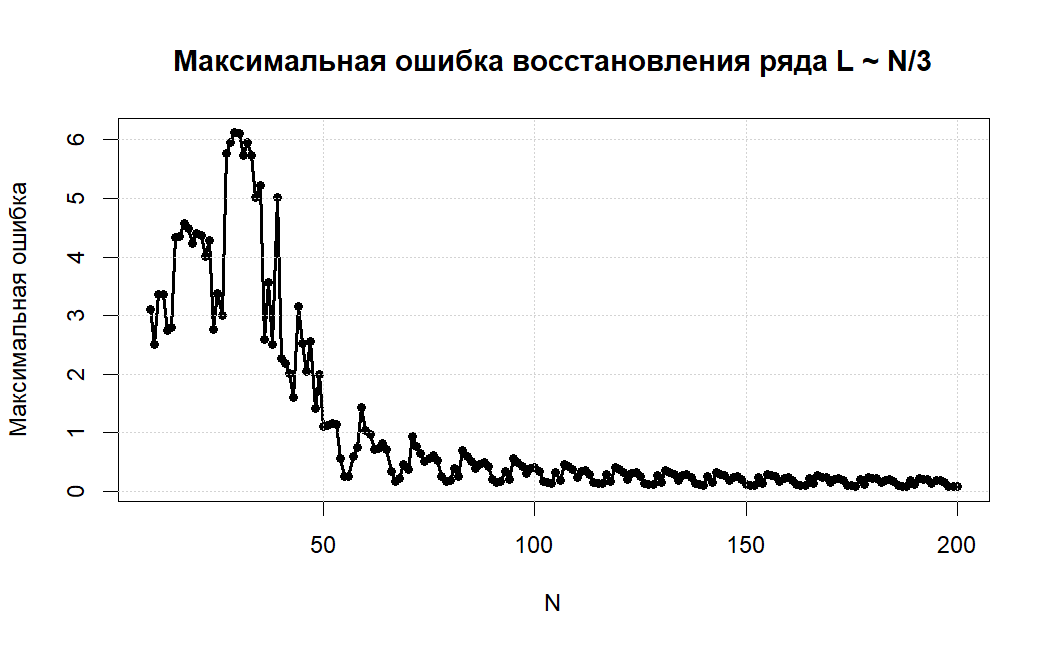
\includegraphics[width=0.95\textwidth]{Pictures/MERNoN.png}
	\caption{Максимальные ошибки восстановления ряда в зависимости от длины ряда при $\widetilde{h}_n = n + 3\cos(\pi n/2 + \pi/8)$.}\label{pic:1}
\end{figure}
\begin{figure}[!h]
	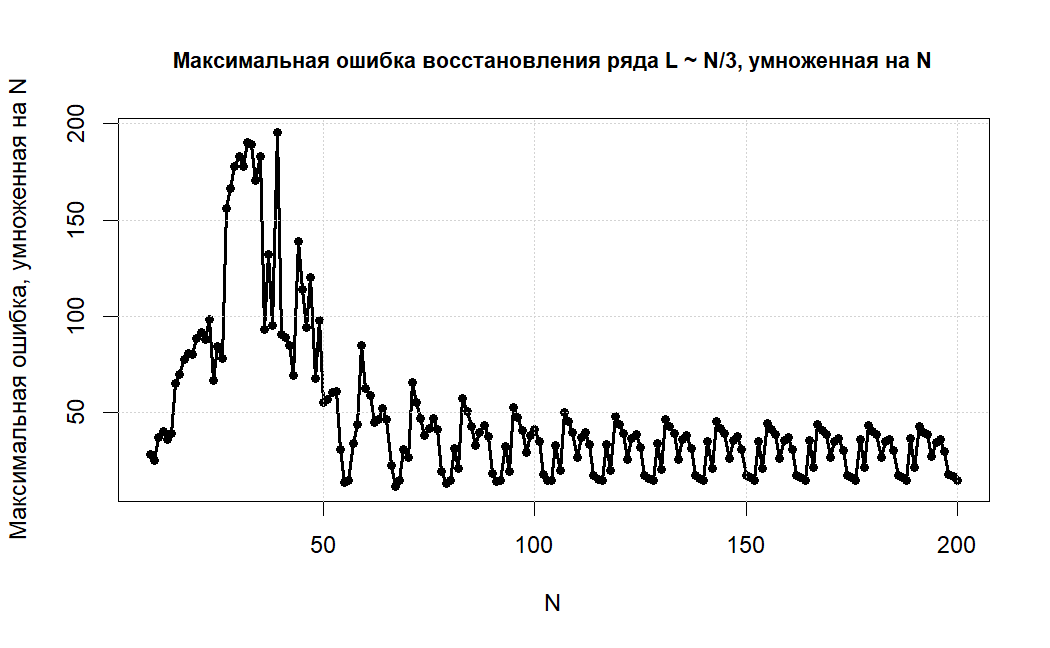
\includegraphics[width=0.95\textwidth]{Pictures/MERN.png}
	\caption{Максимальные ошибки восстановления ряда, умноженные на N, в зависимости от длины ряда N для $x_n = n + 3\cos(\pi n/2 + \pi/8)$.}\label{pic:2}
\end{figure}
\clearpage
Прокомментируем результаты вычислительного эксперимента: по рисунку \ref{pic:1} убедимся, что максимальные по модулю ошибки восстановления ряда стремятся к нулю с ростом N. Рисунок \ref{pic:2} демонстрирует, что после умножения ряда рисунка \ref{pic:1} на N максимальные по модулю ошибки восстановления ряда становятся ограниченными, что подтверждает результат обобщения Теоремы \ref{th:3}.
\section{Заключение}
В ходе проделанных работ были изучены теоретические свойства метода SSA, поставлена общая теоретическая задача, дана оценка $\norm{\mathbf{P}_0^\bot(\delta) - \mathbf{P}_0^\bot - \sum\limits^n_{p=1}\mathbf{W}_p(\delta)}$, а также обобщён случай асимптотической разделимости линейного сигнала с линейной комбинацией гармоник с $L=K$ до $L/N\rightarrow\alpha\in(0,1)$, а также проделан вычислительный эксперимент, подтверждающий результаты обобщения Теоремы \ref{th:3}. 

\bibliographystyle{ugost2008}
\bibliography{report_SSA}
\end{document}
























